\documentclass[11pt,letterpaper]{article}
\usepackage[margin=1.2in]{geometry}
\usepackage{amsmath, amssymb}
\usepackage{times}
\usepackage[mathscr]{euscript}
%\usepackage{mathrsfs}
\usepackage{graphicx}
\usepackage{color}
\usepackage[normalem]{ulem}
\usepackage{bm}
\usepackage{epstopdf}
\numberwithin{equation}{section}
\usepackage{mathrsfs}
\usepackage[round]{natbib}
\usepackage{subcaption}
\graphicspath{ {images/} }
 \usepackage[table]{xcolor}
\usepackage{longtable}
\usepackage[margin=1.2in]{geometry}
\usepackage{amsmath, amssymb}
\usepackage{amsthm}
\usepackage{times}
\usepackage[mathscr]{euscript}
%\usepackage{mathrsfs}
\usepackage{graphicx}
\usepackage{color}
\usepackage[normalem]{ulem}
\usepackage{bm}
\usepackage{epstopdf}
\numberwithin{equation}{section}
\usepackage{mathrsfs}
\usepackage[round]{natbib}
\usepackage{subcaption}
\graphicspath{ {images/} }
 \usepackage[table]{xcolor}
\usepackage{longtable}
\usepackage{array}
\usepackage{relsize}
\usepackage{pdflscape}
\usepackage[margin=1.2in]{geometry}
\usepackage{amsmath, amssymb}
\usepackage{times}
\usepackage[mathscr]{euscript}
%\usepackage{mathrsfs}
\usepackage{graphicx}
\usepackage{color}
\usepackage[normalem]{ulem}
\usepackage{bm}
\usepackage{epstopdf}
\numberwithin{equation}{section}
\usepackage{mathrsfs}
\usepackage[round]{natbib}
\usepackage{subcaption}
\graphicspath{ {images/} }
 \usepackage[table]{xcolor}
\usepackage{longtable}
\usepackage{array}
\newcolumntype{P}[1]{>{\centering\arraybackslash}p{#1}}
\usepackage{changepage}
\usepackage[affil-it]{authblk}
\usepackage{multirow, booktabs}
\usepackage{multicol}
\usepackage[nodisplayskipstretch]{setspace}

\usepackage{bbm}

\begin{document}
\title{\bf Modeling  Frequency and Severity of Claims with the Generalized  Cluster-Weighted Model}

\author{N. Po\v cu\v ca, T. Miljkovic,  P. Jevti\' c, P. McNicholas  }%Nik: need to add names here.

\maketitle
\doublespacing
\small

\begin{abstract}

In this paper, we propose a generalized cluster-weighted  model (GCWM) that allows for modeling non-Gaussian distribution of the continuous covariates. Additionally, our zero-inflated GCWM allows for modeling zero-inflated cluster weighted distribution of claims that is more suitable in the insurance applications. We describe an expectation-optimization (EM) algorithm for parameter estimation in GCWM. Cluster-weighted models are considered as a flexible family of mixture models for fitting the joint distribution of a random vector composed of a response variable and a set of continues and discrete covariates. However, these models have a few limitations when it comes to the insurance applications and may provide suboptimal results. A simulation study showed that the GCWM a performs well for different settings in contrast to the existing mixture-based approaches. A real data set based on French auto-mobile policies is used to illustrate the application of the proposed model.

\end{abstract}
\textsc{Key Words:} finite mixture models, GLM, GCWM a, CWM, ratemaking, automobile claims.\\
\textsc{JEL Classification:}  C02, C40, C60.\\
% C02-Mathematical Methods, C40-General mathematical and statistical methods: special topics, c60-General mathematical methods, programming models, mathematical and simulation modeling%
\section{Introduction}\label{sec:introduction}
Predictive modeling gained a lot of attention in the past decade in the area of actuarial science, risk management, and insurance in general. While the term predictive modeling has been used in many other areas, in context of insurance, it is referred to as a process of leveraging statistics in estimating the insurance cost \citep[see][]{Frees+Derrig+Meyer:2014}. Various predictive models are used in the area of actuarial science with generalized linear models (GLMs) being the most popular tools actively integrated in pricing, reserving, and underwriting of property and casualty insurance. The most recent extensions of the GLM models proposed by \cite{Garrido+Genest+Schulz:2016} and \cite{Shi+Feng+Ivantsova:2015} allow for relaxing the assumption of independence between number and size of claims. Several GLM extensions based on copulas have been considered \citep[e.g.,][]{Frees+Lee+Yang:2016,Kramer+Brechmann+Silvestrini+Czado:2013, Czado+Kastenmeier+Brechmann+Min:2012,Frees+Wang:2006}.


\cite{Ingrassia+Punzo+Vittadini+Minotti:2015} proposed a cluster-weighted models (CWMs) as a flexible family of mixture models for fitting the joint distribution of a random vector composed of a response variable and a set of mixed-type covariates with the assumption that continues covariates come from Gaussian distribution. In this paper paper, we consider two extensions of CWM model to allow modeling of non-Gaussian continues covariates and a zero-inflated Poisson (ZIP) claims distribution. We define our proposed model as cluster-weighted transformed model or GCWM a which is more suitable for the insurance applications.
%
The CWM models with Gaussian assumptions have been proposed by \cite{Gershenfeld:1997}, \cite{Gershenfeld:Schoner+Metois:1999}, and \cite{Gershenfeld:1999} in a context of media technology. Some extensions of this class of models have been considered by \cite{Punzo+Ingrassia:2015}, \cite{Ingrassia+Minotti+Punzo:2014}, and \cite{Ingrassia+Minotti+Vittadini:2012}.

There is a growing interest in modeling insurance losses using mixture models. Several recent mixture models of univariate insurance data have been developed, including work by \cite{Lee+Lin:2010}, \cite{Verbelen+Gong+Antonio+Badescu+Lin:2015}, and \cite{Miljkovic+Grun:2016}. A finite mixture of bivariate Poisson regression models with an application to insurance ratemaking was studied by \cite{Bermudez+Karlis:2012}. The authors used the EM algorithm to determine the number of components in the mixture. Another Poisson mixture model for count data was considered by \cite{Brown+Buckley:2015} with application in managing a Group Life insurance portfolio. Motivated by the idea of mixture modeling, we believe that the extension of the univariate mixture modeling can be applied to mixture modeling of regressions including the GLMs, where losses are modeled as a function of several covariates.

This paper is organized as follows. Section 2 presents the proposed model for mixture of GLMs. Section~3 applies the proposed model on a real data of French automobile claims. An extensive simulation study is discussed in Section 4. Conclusion is provided in Section 5.


\section{Proposed Model}

\subsection{Background}

Let $(\bm{X^{'}}, Y)^{'}$  be the pair of a vector of covariates  $\bm{X}$ and a response variable $Y$. Assume this set is defined on some space $\Omega$ that takes values in appropriate Euclidian subspace. Further, assume that there exists $G$ partitions of $\Omega$, denoted as $\Omega_1, \ldots, \Omega_G$.  \cite{Gershenfeld:1997} characterized the Cluster weighted models as a finite mixture of GLMs hence, the joint distribution $f(\bm x, y)$ of $(\bm{X^{'}}, Y )^{'}$  is expressed as follows
 \begin{align}
 f(\bm x, y)= \sum_{j=1}^{G} \tau_j f(y|\bm{x};\Omega_j)f(\bm{x};\Omega_j).
\label{eq1}
\end{align}
\flushleft The pair $f(y|\bm{x};\Omega_j)$ and $f(\bm{x};\Omega_j)$ are conditional and marginal distributions of $(\bm{X^{'}}, Y)^{'}$ respectively, while $\tau_j$ represents the weight of the $j$th component such that $\sum_{j=1}^{G}\tau_j=1$, $\tau_j>0$.
\cite{Ingrassia+Punzo+Vittadini+Minotti:2015} proposed a flexible family of mixture models for fitting the joint distribution of a random vector $(\bm{X^{'}}, Y)^{'}$ by splitting the covariates into continues and discrete as $ \bm{X}=(\bm{V^{'}},  \bm{W^{'}})^{'}$. This assumption of independence between continues and discrete covariates allows us to multiply their corresponding marginal distributions. Thus, for this setting the model in \eqref{eq1} is reformulated as follows
\begin{align}
 f(\bm x, y; \Phi)= \sum_{j=1}^{G} \tau_j f(y|\bm{x};\bm{\vartheta_j})f(\bm{x};\bm{\theta_j})=\sum_{j=1}^{G} \tau_j f(y|\bm{x};\bm{\vartheta_j})f(\bm{v}; \bm{\theta_j^{\star}})f(\bm{w};\bm{\theta_j^{\star\star}})
\label{eq2}
\end{align}
where $\bm{v}$ and $\bm{w}$ are the vectors of continues and discrete covariates respectively, the $f(y|\bm{x};\bm{\vartheta_j})$ is a conditional density of $Y|\bm{x}$, with parameter vector $\bm{\vartheta_j}$, the $f(\bm{v};\bm{\theta_j^{\star}})$ is the marginal distribution of $\bm{v}$ with parameter vector $\bm{\theta_j^{\star}}$. the $f(\bm{w};\bm{\theta_j^{\star\star}})$ is the marginal distribution of $\bm{w}$ with parameter vector $\bm{\theta_j^{\star\star}}$. Finally $\bm{\Phi}:=(\bm{\theta^{\star}},\bm{\theta^{\star\star}}, \bm{\tau}, \bm{\vartheta})$ includes all model parameters. %Nik: this does not seem to be all model parameters? Also, vartheta is either bold face (vector) or not (scalar), and what is $\lm$?. % Notation Corrected - Nik
In addition, the conditional distribution $f(y|\bm{x};\bm{\vartheta_j})$ is assumed to belong to an exponential family of distributions and as such can be modeled in the framework of GLMs. Here, the marginal distribution of continues covariates is assumed to be Gaussian type. Unfortunately, this assumption is too strong for using insurance related applications specifically in rate-making. To relax this constraint, we develop a new model that allows for modeling of non-Gaussian covariates as discussed in the next section.

\subsection{Generalized cluster-weighted model (GCWM) }
We proceed to extend \eqref{eq2} by splitting the  continues covariates further as $\bm{V}:=(\bm U^{'}, \bm T^{'})^{'}$, where $\bm{U}$ is a set of non-Gaussian covariates, and $\bm{T}$ as a set of Gaussian  covariates.  Thus (\ref{eq2}) is now recovered as
\begin{align}
 f(\bm x, y; \Phi)= \sum_{j=1}^{G} \tau_j f(y|\bm{x};\bm{\vartheta_j})f(\bm{t};\bm{\theta_j^{\star}})f(\bm{w};\bm{\theta_j^{\star\star}})f(\bm{u};\bm{\theta_j^{\star\star\star}})
\label{eq3}
\end{align}
where $f(\bm{t};\bm{\theta_j^{\star}})$ represents the marginal density of Gaussian covariates, with parameter vector $\bm{\theta^{\star}}$, and $f(\bm{u};\bm{\theta_j^{\star\star\star}})$ as the marginal density of the non-Gaussian covariates with parameter vector $ \bm{ \theta_j^{\star\star\star}} $.


As it is relevant to most actuarial applications in this paper, we focus on the  log-normal distribution  for non-Gaussian covariates. Hence, with our log-normal assumption for $f(\bm{u};\bm{\theta_j^{\star\star\star}})$, we have that $\bm{u}$ is defined on $\mathbb{R}^+$ with parameter vector $ \bm{\theta_j^{\star\star\star}} $, and having marginal density
\begin{align} f \left(  \bm{u}; \bm{\theta_j^{\star\star\star}} := ( \bm{\mu_j^\star} ,\bm{ \Sigma _j^\star } ) \right) = \frac{1}{(\prod_{i=1}^{N}u_{i})|\bm{ \Sigma_j^\star} |(2 \pi)^{\frac{p}{2}}}   \exp\left[-\frac{1}{2}(\ln\bm{ u}-\bm{\mu_j}^\star)^{'}\bm{\Sigma_j^{-1}}(\ln \bm {u}-\bm{\mu_j}^\star)\right].
\end{align} The derivation of the multivariate log-normal distribution can be found in the Appendix \ref{changeVarUni}.

%Nik: is this a density? What range of values of x? What values can mu and sigma take? 
% PM: Is this more clear?

\subsection{Zero-inflated Poisson}%Nik: not sure what this means? Specifically, what is the role of the first "-"

For the zero-inflated Poisson model (ZIP) see \cite{Lambert} we can split the conditional density $f(y|\bm{x},\bm{\vartheta_j})$ into zero and non-zero densities. %Nik: I don't think "groups" is what is meant.  % Values I meant. 
The response $y$ variable when $y= 0$  are distributed with density $f(0|\bm{x},\bm{\vartheta_{j}})$. The response $y$ values when $y > 0$ are distributed with density $f(y > 0|\bm{x}, \bm{\vartheta_{j}} )$. Given the conditional density now defined for the ZIP model, \eqref{eq3}   
can be re-written as follows 
 \begin{align}
 f(\bm x, y; \Phi)= \sum_{j=1}^{G} \tau_j \left[ f(0|\bm{x};\bm{\vartheta_{j} }) +  f(y > 0|\bm{x} ; \bm{\vartheta_{j}})  ) \right]   f(\bm{t};\bm{\theta_j^{\star}})f(\bm{w};\bm{\theta_j^{\star\star}})f(\bm{u};\bm{\theta_j^{\star\star\star}}). 
\end{align}

\newcommand{\xTilda}{\bm{\tilde{x}}}
Let $ \xTilda := [\bm{1},\bm{x}]$, where $\xTilda $ is a matrix of covariates with the addition of a placeholder for the intercept in the GLM. We denote the Poisson conditional density  as $ f^P(y|\bm{x}; \bm{\beta_j}) $, where $y \in \{0,1,\dots\}$, and  $\bm{\beta_j}$ is the row coefficient vector. 
Here, the link function will be modelled with log-link for the GLM:
 \begin{align*}
\lambda_j = e^{\xTilda \bm{\beta_j}'}, && %\beta_{0j} + \beta_j^{'}x
f^P(y|  x ; \lambda_{j} ) = e^{-\lambda_j} \frac{{\lambda_j}^y}{y!}.
 \end{align*}
Next, we introduce a Bernoulli process for the conditional density but first we introduce a new indicator function $\mathbbm{1}(\cdot) $, where 
	\begin{align*}
	\mathbbm{1}(y) = \begin{cases}
	 1, & y = 0\\
	 0, & y \neq 0. 
	\end{cases}
	\end{align*} We denote the density as  $ f^{B}(y|\bm{x}; \bm{\bar{\beta_j}}) $, where $\mathbbm{1}(y) \in \{0,1 \} $, and  $\bm{\bar{\beta_j}}$ as the coefficient vector.  Here, the GLM will be modeled with the associated logit link function
 \begin{align*}
 \psi_j =  \frac{e^{\xTilda \bm{\bar{\beta_j}}'}}{1+ e^{\xTilda  \bm{\bar{\beta_j}}'}},  &&
 f^B(y | \bm{x} ; \bm{\bar{\beta_j}}) = \begin{cases} 
      \quad \psi_j, & \mathbbm{1}(y) = 0 \\
     1 -  \psi_j,  & \mathbbm{1}(y) = 1
   \end{cases}
 \end{align*}
 Now, given a combination of two preceding models, we introduce the ZIP process in which zero counts come from two random variables. One comes from Bernoulli random variable which generates structural zeros, and the other comes from the Poisson random variable. The coefficients $ \bm{\vartheta_{j}} :=  \{ \bm{\beta_{j}},  \bm{\bar{\beta_j}} \} $ correspond to the two above introduced conditional densities where the coefficients are estimated using a generalized linear model as in \cite{Lambert}. The components of ZIP conditional density $f(y|\bm{x}; \bm{\vartheta_{j}}  )$ are %Nik: something missing here?, PM: Fixed.
 \begin{align*}
 f(0 | x ; \bm{ \vartheta_{j} } ) = \psi_j + (1 - \psi_j)e^{-\lambda_j}  & &  \text{and}  & &
f(y > 0 |  x ; \bm{ \vartheta_{j} } ) = (1 - \psi_j)e^{-\lambda_j} \frac{\left(\lambda_j \right)^y  }{y!}.  
 \end{align*}
Also, the link functions to consider are log-link for the Poisson process and logit link for the Bernoulli
 \begin{align*}
 \psi_j =  \frac{e^{\xTilda \bm{\bar{\beta_j}}'}}{1+ e^{\xTilda \bm{\bar{\beta_j}}'}}  & & \text{and} & &
\lambda_j  = e^{\xTilda \bm{\beta_j}'}.
 \end{align*}

Let paramater $\psi_j$ denote the probability that the zero comes from the Bernoulli distribution of $j$th component, and the parameter $ \lambda_j $ characterizes the $j$th Poisson distribution. This allows for a more nuanced approach to handling the inflation of zeros similarly as in \cite{Bermudez+Karlis:2012}.  
\section{Introducing Bernoulli-Poisson Partitioning}

The single component ZIP model assumes that the inflated zeros emanate from both a Bernoulli and Poisson random variables while the non-zeros are assumed to come exclusively from the Poisson random variable. However, recent research  extends the single component ZIP models to mixture models for heterogeneous count data with excess zeros (see  \citep{Bermudez+Karlis:2012}). In mixtures of ZIPs, zeros are assumed to come from multiple different Binomial and Poisson random variables.  Difficulties are apparaent  during the maximization step of the EM when means of covariates are very close together (see  \cite{LimHwa}) . However, misclassification error can be reduced using parsimonious models for the indepedent variables as in  \cite{McNicholas:2010}. 

	In this work, we propose a new method to rectify this problem and partition the dataset using Bernoulli and Poisson GCWMs. Furthermore, we construct a new zero inflated GCWM (ZI-GCWM) using the previously generated Bernoulli and Poisson GCWMs. We show that the Bernoulli and Poisson GCWM accurately estimate the initialization of the EM algorithm for the zero inflated GCWM model. The work of \cite{Lambert} specifies that the MLE estimates for coefficients provide an excellent guess allowing EM to converge quickly for ZIPs. The partitioning method consists of two seperate EM algorithms. The first EM algorithm is for generating the GCWM models, while the second EM is for optimizing the ZI-GCWM. Recall $(\bm {X^{'}}, Y)^{'}$ to be a vector defined on some sample space $\Omega$. As discussed, this sample space is partitioned into $G$ non-overlapping sets such that their union constitutes this sample space ie. $ \Omega = \bigcup_{i=1}^G \Omega_i $.  However, contingent on a model choice each particular set $\Omega_i$ may take a different shape. 
	 Specifically, if we introduce the Bernoulli model in a generalized form for conditional density (see \cite{Ingrassia+Punzo+Vittadini+Minotti:2015} for specific cases), we have the sample space $\Omega^B$ and joint pdf $f^B$ to be \begin{align*} 
\Omega^B =  \bigcup_{l =1}^G \Omega_l^B & & \text{and} &  &
f^B(\bm x, y; \Phi)= \sum_{l=1}^{G} \tau_l f^B(y|\bm{x}; \bm{\bar{\beta_l}}) f(\bm{t};\bm{\theta_l^{\star}})f(\bm{w};\bm{\theta_l^{\star\star}})f(\bm{u};\bm{\theta_l^{\star\star\star}}). 
\end{align*} 
Similarly if we introduce a Poisson model in a generalized form the sample space $\Omega^P$ and joint pdf $f^P$ become
\begin{align*}
\Omega^P =  \bigcup_{j =1}^M \Omega_j^P & & \text{and} &  &
f^P(\bm x, y; \Phi)= \sum_{j=1}^{M} \tau_j f^P(y|\bm{x};\bm{\beta_{j}}) f(\bm{t};\bm{\theta_j^{\star}})f(\bm{w};\bm{\theta_j^{\star\star}})f(\bm{u};\bm{\theta_j^{\star\star\star}}).  
\end{align*}
Where this sample space is partitioned up to M non-overlapping sets. 
 Now, construct a new partitioning of a sample space $\Omega$ such that 
$$\Omega =  \Omega^Z = \bigcup_{l \in \{1 \ldots G \} , j \in \{1 \ldots M \}  } \Omega_{l,j}^Z := \bigcup_{l \in \{1 \ldots G \} , j \in \{1 \ldots M \}  }  \Omega_l^B \cap \Omega_j^P := \bigcup_{k \in \{1 \ldots K \}} \Omega_k^Z $$, where $K$ can range up to $M \times G$ unique partitions. Therefore the new conditional density  is now result of a model in which each component is captured by the conditional pdf that is of mixture of particular Bernoulli and particular Poisson
\begin{align} 
f^Z_{k}(y|\bm{x};  \bm{\bar{\beta}}_k,\bm{ \beta}_k) := f^B(y|\bm{x}; \bm{\bar{\beta}}_k) +(1-  f^B(y|\bm{x}; \bm{\bar{\beta}}_k) ) f^P(y|\bm{x};\bm{\beta}_k).
\label{initialziGCWM}\\ 
= f(0|\bm{x};\bm{\vartheta_{k} }) +  f(y > 0|\bm{x} ; \bm{\vartheta_{k}})
\label{ziGCWM} 
\end{align}


The expectation-maximization (EM) algorithm (see \cite{Dempster+Laird+Rubin:1977}) is then used to estimate this new mixture of up to $M \times G$ specific GCWMs. The initialization parameters for the second EM algorithm are provided by Bernoulli and Poisson GCWMs from \eqref{initialziGCWM} giving parameter pairs ($ \psi_k,\lambda_k  $) where $k \in \{1 \dots K \} $. The second EM procedure then optimizes \eqref{ziGCWM}. The ZI-GCWM is then compared against the standard Poisson GCWM using a modified test which is commented in section 3.6. 

\subsection{The EM Algorithm for Parameter Estimation}
In most finite mixture problems, the standard method for estimating parameters of mixture models is based on the EM algorithm and further discussed by \cite{McLachlan+Peel:2000}.
The Bernoulli-Poisson partitioning method is split into two EM algorithm steps. The first EM partitions the sample space, while the second EM optimizes the zero inflated portion. 
 %Nik: this is incorrect. The EM algorithm does not estimate the optimal number of components.  PM: Removed.
 \subsection{EM - Partitioning}
 
The EM algorithm is based on the local  maximum likelihood estimation. %Nik: need to be careful here. Please reword. , PM: Local maximum?  
The initial values of the parameter estimates can be generated from a variety of strategies outlined in \cite{initialPaperGrassiaRef}, %Nik: this may or may not be the case. 
% PM: I cited the same paper ingrassia used for initializations. 
then the algorithm proceeds by alternation of the E-step and M-step to update parameter estimates. %Nik: again, need to be much more careful. 
To find an optimal number of components, maximum likelihood estimation is obtained over a range of $G$, and the best model is selected based on the Bayesian information criterion (BIC).   %Nik: which one? Explain. %PM: BIC was used. 

The convergence criterion of the EM algorithm is based on the Aitken acceleration. It is used to estimate the asymptotic maximum of the log-likelihood at each iteration of the EM algorithm.  when the relative increase in the log-likelihood function is no bigger than a small pre-specified tolerance value or the number of iterations reach a limit. %Nik: that is a possible stopping rule but is not a convergence criterion per se.
In this subsection, we explain the parameter estimation in line with the GCWM methodology proposed by \cite{Ingrassia+Punzo+Vittadini+Minotti:2015}. The proposed GCWM a model is based on the assumption that $f(y|\bm{x},\vartheta_j)$ belongs to the exponential family of distributions that are strictly related to GLMs. The link function relates the expected value $g(\mu_j)= \beta_{0j} + \beta_{1j} x_{1}+ \cdots+\beta_{pj} x_{p}$. We are interested in estimation of the vector $\bm \beta_j$, thus the distribution of $y|\bm{x}$ is denoted by $f(y|\bm{x}; \bm{\beta_j}, \lambda_j)$, where $\lambda_j$ denotes an additional parameter to account for when a distribution belong to a two-parameter exponential family.

The marginal distribution $f(\bm{x}; \bm \theta_j)$ has the following components: $f(\bm{t}; \bm \theta_j^{\star})$, $f(\bm{w}; \bm \theta_j^{\star\star})$, and $f(\bm{u};\bm \theta_{j}^{\star\star\star})$. The first marginal density $f(\bm{t}; \bm \theta_j^{\star})$ is modeled as a  Gaussian with mean $\bm {\mu_j}$ and covariance matrix $\bm \Sigma_j$ as $f(\bm t; \bm {\mu_j}, \bm \Sigma_j)$. The marginal density $f(\bm{w};\bm \theta_{j}^{\star\star})$ assume that each finite discrete covariate $W$ is represented as a vector $\bm{w}^r=(w^{r1},\ldots,\bm{w}^{rc_r})^{'}$ where $w^{rs}=1$ if $w_r = s$, such that $s\in\{1, \ldots, c_r\}$, %Nik: this wording seems very awkward. Does "has the value" just mean "="? If so, why not write "="?
and $w^{rs}=0$ otherwise.
%Nik: the previous sentence does not make sense to me, and the following equation seems to come out of nowhere.
\begin{align}
f(\bm {w}, \bm {\gamma_j})=\prod_{r=1}^{q}\prod_{s=1}^{c_r}(\gamma_{jrs} )^{w^{rs}} 
\label{eq31}
\end{align}
for $j=1, \ldots, G$, where $\bm {\gamma_j}=(\gamma_{j1}^{'}, \ldots, \gamma_{jq}^{'})^{'}$, $\bm \gamma_{jr}=(\gamma_{jr1}^{'}, \ldots, \gamma_{jrc_q}^{'})^{'}$, $\gamma_{jrs} > 0$, and  $\sum_{s=1}^{c_r}\gamma_{jrs}$, $r=1,\ldots,q$. The density $f(\bm {w}, \bm{\gamma_j})$ represents the product of $q$ conditionally independent multinomial distributions with parameters $\bm{\gamma}_{jr}$, $r=1,\ldots, q$. The last marginal density $f(\bm{u};\bm \theta_{j}^{\star\star\star})$ will be modelled as lognormal with mean vector $ \bm \mu_j^\star$, and covariance matrix $\bm \Sigma_j^\star $. 

Let $(\bm x_1, y_1),\ldots, (\bm x_n, y_n)$ be a sample of $n$ independent observations drawn from model in \eqref{eq3}.
For this sample, the complete data likelihood function, $L_c(\bm\Phi)$, is given by
\begin{align}
L_c(\bm\Phi)=\prod_{i=1}^{n}\prod_{j=1}^{G}\left[{\tau_j}f(y_i|x_i, \bm \beta_j, \lambda_{j})f(t_i, \bm\mu_j, \bm\Sigma_j) f(w_i, \gamma_j)f(u_i, \bm{\mu_j}^\star,\bm{\Sigma_j}^\star) \right]^{z_{ij}},
\label{eq27}
\end{align}
where $z_{ig}$ is the latent indicator variable with value of $z_{ig}=1$ indicating that observation $(\bm{x_i}, y_i)$, originated from the $j$th mixture component and $z_{ij}=0$ otherwise.

By taking the logarithm of \eqref{eq27}, the complete-data log-likelihood function $\ell_c(\bm\Phi)$ is written by
\begin{equation*}\begin{split}
\ell_c(\bm\Phi)= \sum_{i=1}^{n}\sum_{j=1}^{G}{z_{ij}}\big[\log(\tau_{j}) + \log{f}(y_i|x_i,\bm \beta_j,\lambda_j)+ \log f(t_i, \bm\mu_j, \bm\Sigma_j) & + \log f(w_i, \gamma_j)\\& +\log {f}(u_i, \bm{\mu_j}^\star,\bm{\Sigma_j}^\star) \big].
\label{eq28}
\end{split}\end{equation*}

\subsubsection{E-Step - Partitioning}
The $E$-step does not depend on the form of density, and the latent data only relate to $\bm z$. %Nik: please reword 
The posterior probability that $(\bm{x_i}, y_i)$ comes from the $j$th mixture component is calculated at the $s$th iteration of the EM algorithm as
\begin{equation*}\begin{split}
    {\pi_{ij}}^{(s)} &= {E}[z_{ij} |(\bm{x_i}, y_i), \bm{\Phi}^{(s)}]\\
     &= \frac{{\tau_j}^{(s)}f(y_i|x_i, \bm \beta_j^{(s)}, \lambda^{(s)}_{j})f(t_i, \bm\mu_j^{(s)}, \bm\Sigma_j^{(s)}) f(w_i, \gamma_j^{(s)})f(u_i, \bm{\mu_j}^{\star (s)},\bm{\Sigma_j}^{\star (s)})}{f(\bm{x_i}, y_i; \Phi^{(s)})
\label{eq29}                       }.
\end{split}\end{equation*}
\subsubsection{M-Step - Partitioning} 
It follows that at the $(s+1)$th iteration, the conditional expectation of \eqref{eq28} on the observed data and the estimates from the $s$th iteration results in
\begin{multline}
Q(\bm\Phi|\bm\Phi^{(s)}) = \sum_{i=1}^{n}\sum_{j=1}^{G}{\pi_{ij}^{(s)}} \big[\log(\tau_{j}) + \log{f}(y_i|x_i,\bm \beta_j,\lambda_j)+ \log f(t_i, \bm\mu_j, \bm\Sigma_j)  + \log f(w_i, \gamma_j) +\log {f}(u_i, \bm{\mu_j}^{\star (s)},\bm{\Sigma_j}^{\star (s)})\big] \\
=\sum_{i=1}^{n}\sum_{j=1}^{G}{\pi_{ij}^{(s)}}\log(\tau_{j}) + \sum_{i=1}^{n}\sum_{j=1}^{G}{\pi_{ij}^{(s)}}\log{f}(y_i|x_i,\bm \beta_j^{(s)},\lambda_j^{(s)}) +\sum_{i=1}^{n}\sum_{j=1}^{G} {\pi_{ij}^{(s)}}\log f(t_i, \bm\mu_j^{(s)}, \bm\Sigma_j^{(s)}) \\
+\sum_{i=1}^{n}\sum_{j=1}^{G}{\pi_{ij}^{(s)}}\log f(w_i, \gamma_j^{(s)}) + \sum_{i=1}^{n}\sum_{j=1}^{G}{\pi_{ij}^{(s)}}\log {f}(u_i, \bm{\mu_j}^{\star (s)},\bm{\Sigma_j}^{\star (s)}).\label{Qfunction}
\end{multline}


The M-step requires maximization of the $Q$-function with respect to $\bm \Phi$ which can be done separately for each term on the right hand side in \eqref{Qfunction}. %Nik: first, I don't see a (2.11); second, use \eqref{} 
As a result, the parameter updates $\hat{\tau}_j$, $\hat{\bm \mu^{}}_j$, $\hat{\bm \sigma}_j$, and $\hat{\bm \gamma}_j$ on the $(s+1)$th iteration are:
\begin{align*}
{\hat{\tau}_j}^{(s+1)}&=\frac{1}{n} \sum_{i=1}^n \pi_{ij}^{(s)}, && && {\hat{\bm \mu^{}}_j}^{(s+1)}=\frac{1}{\sum_{i=1}^n \pi_{ij}^{(s)}} \sum_{i=1}^n \pi_{ij}^{(s)}\bm t_i, &&  && {\hat{\bm \gamma}^{(s+1)}_{jr}} =\frac{\sum_{i=1}^n \pi_{ij}^{(s)} \omega^{rs}_i} {\sum_{i=1}^n \pi_{ij}^{(s)}}, 
\end{align*}
$$
 {\hat{\bm \sigma^{}}_j}^{(s+1)}=\frac{1}{\sum_{i=1}^n \pi_{ij}^{(s)}} \sum_{i=1}^n \pi_{ij}^{(s)}(\bm t_i-\hat{\bm \mu}^{(s+1)}_j) (\bm t_i-\hat{\bm \mu}^{(s+1)}_j)^{'}  ,
$$

The log-normal distribution is relevant for modelling actuarial data.  Parameter estimates for the log-normal distribution follow similar suit.
\begin{align*}
{\hat{\tau}_j}^{(s+1)}&=\frac{1}{n} \sum_{i=1}^n \pi_{ij}^{(s)},&&
{\hat{\bm \mu}_j}^{\star (s+1)}=\frac{1}{\sum_{i=1}^n \pi_{ij}^{(s)}} \sum_{i=1}^n \pi_{ij}^{(s)}\ln \bm u_i,&&
\end{align*}
$$ {\hat{\bm \sigma^{}}_j}^{\star(s+1)}=\frac{1}{\sum_{i=1}^n \pi_{ij}^{(s)}} \sum_{i=1}^n \pi_{ij}^{(s)}(\ln \bm u_i-\hat{\bm \mu}^{\star(s+1)}_j) (\ln \bm u_i-\hat{\bm \mu}^{\star(s+1)}_j)^{'}. $$

The estimates of $\bm\beta$ are computed by maximizing each of the $G$ terms
\begin{align}
\sum_{i=1}^{n}\pi^{(s)}_{ij} \log{f}(y_i|\bm x_i,\bm \beta_j,\lambda_j).
\label{eq30}
\end{align}
Maximization of \eqref{eq30} is performed by numerical optimization in R software in a similar framework the mixture of generalized linear models are implemented. For additional details about this implementation the reader is refer to \cite{Wedel+DeSabro:1995} and \cite{Wedel:2002}.
For insurance applications, current TCWM model can be used for modeling frequency of claims assuming that $\bm{Y}$ belongs to Poisson or Bernoulli distributions. When modelling severity of claims, $\bm{Y}$ can be assumed accommodate Gamma or Lognormal distributions. All of these applications are based on CWM as the underlying approach. For additional information, the reader is referred to the manual of the {\tt flexCWM} package manual for ${\bf R}$ users written by \cite{Ingrassia+Punzo+Vittadini+Minotti:2015}.%Nik: use \cite
\subsection{EM - Zero-inflated}
The optimization of the zero-inflated model uses the EM algorithm to maximize the incomplete-data log-liklihood iteratively \citep{Lambert}. The log-likilhood for $\psi_k$ and $\lambda_k$ is expressed as 

\begin{align*}
l(\psi_k,\lambda_k; y, \bm{x}) = \sum_{y_i = 0} \log \big[ e^{ \bm{ \xTilda_i \bar{\beta}_k^{'} } } + \exp{( - e^ { -\bm{ \xTilda_i \beta_k^{'} }})} \big] + \sum_{y_i > 0 } \left( y_i \xTilda_i \bm{\beta_k}^{'} + e^{ \xTilda_i \bm{\beta_k}^{'} } \right) - \sum_{i=1}^n  \log \left(1 + e^ {\xTilda_i \bar{\beta_k}^{'} } \right) - \sum_{y_i > 0} \log(y_i ! )
\end{align*}

Where $y_i$, and $\xTilda_i$ referes to the ith row of the response variable $y$ and covariate matrix $\xTilda$. Due to the first term, the log-liklihood is complicated to maximize, \cite{Lambert} provides a meaningful solution. Suppose that we could observe $\bm{Z_i} = 1$ when $y_i$ is generated from the Bernoulli random variable, and $\bm{Z_i} = 0$ when $y_i$ is generated from the Poisson random variable. Then the complete-data log-liklihood would be written as

\begin{align}
l_c(\psi_k,\lambda_k;y,\bm{z }) = & \sum_{i=1}^n \left( \bm{z_i\xTilda_i \bar{\beta_k }^{'}} - \log(1+ e^{\bm{ \xTilda_i \bar{\beta_k }^{'}}} \right) + \sum_{i=1}^n (1-\bm{z_i}) (y_i \bm{ \xTilda_i \beta_k^{'} } - e^{\bm{\xTilda_i \beta_k^{'}}}) + \sum_{i=1}^n (1-\bm{z_i})\log(y_i!) \nonumber \\
=  & \quad l_c(\psi_k;\bm{y,z}) + l_c(\lambda_k; \bm{y,z}) + \sum_{i=1}^n (1-\bm{z_i})\log(y_i!) \label{CompleteZLog}
\end{align}

where $\bm{z_i}$ is a realization of $\bm{Z_i}$. \eqref{CompleteZLog} is easier to maximize since $l_c(\psi_k;\bm{y,z})$ and $l_c(\lambda_k; \bm{y,z}) $ can be maximized seperately for parameters $\lambda_k$ and $\psi_k$. With the EM algorithm, the incomplete-data log-liklihood can be maximized iteratively between estimating $Z_i$ with its expectation under current parameters $\lambda_k$ and $\psi_k$ (E-Step) and then maximizing the complete data-logliklihood (M-Step). 

\subsubsection{E-step -  Zero-inflated}%Nik: again, why the first "-"?
 % PM: There are two EzM algorithms, one is used to partition the dataset, the other EM is to optimize the Zero inflated cond density. 

Using current estimates $\psi_k^{(s)}$ and $ \lambda_k^{(s)} $ from the partition $ \Omega_{Z_k}$, we calculate the expected value of $Z_i$ by its posterior mean $z_i^{(s)}$ for each cluster, at iteration s
\begin{align*}
z_{i}^{(s)} = \begin{cases}  \left[ 1 + \exp{\big(-\bm{\xTilda_i \bar{\beta_k}^{'(s)}} - e^ {\bm{\xTilda_i \beta_k^{'(s)}}} \big) } \right]^{-1}, &  y_{i} = 0 \\
  0 \quad , & y_{i}> 0 .
\end{cases}
\end{align*}


\subsubsection{M-Step - Zero-inflated}
The M-Step can be split into the maximization of two complete data log-likelihoods and the $\bm{z_i}$ calculated from the previous iteration $(s)$ as: 
\begin{align} 
l_c(\psi_k;\bm{y,z}) &=\sum_{i=1}^n \left( \bm{z_i\xTilda_i \bar{\beta_k }^{'(s)}} - \log(1+ e^{\bm{ \xTilda_i \bar{\beta_k }}^{'(s)}} \right)  \label{eq6}   \\
 l_c(\lambda_k; \bm{y,z}) &= \sum_{i=1}^n (1-\bm{z_i}) (y_i \bm{ \xTilda_i \beta_k^{'(s)} } - e^{\bm{\xTilda_i \beta_k}^{'(s)}})\label{eq7} 
 \end{align}
The maximization of \eqref{eq7} for GLM coefficients $\lambda_k$ can be found by using a weighted, log-linear Poisson regression with weights $1 - z_{ik}^{(s)}$ \citep{McCullaghNelder1989}, yielding $\lambda_k^{(s+1)}$. 
While the parameter for \eqref{eq7} can be maximized over a gradient \citep{Lambert} yielding $\psi_k^{(s+1)}$.

\subsection{Comparing Zero-inflated Models}

The standard test for comparing zero-inflated to non-zero inflated models has been the Vuong Test for non-nested models \citep{vuongTest}. However recent work has shown the misuse of this test for zero inflation \citep{misuse}. \cite{newIntuitive} shows that it is sufficient to test for zero-modificiation in the form of a liklihood ratio test. The test is defined as follows: 
\begin{align*}
& & H_0: \quad \psi_k = 0 \quad\quad vs. \quad\quad H_a: \quad \psi_k \neq 0  & & 
\end{align*}
\begin{align*}
\varphi = -2 \bigg[l(\tilde{\lambda_k}; y, \bm{x}) - l(\lambda_k, \psi_k; y , \bm{x} )\bigg] 
\end{align*}
where $l(\tilde{\lambda_k}; y , \bm{x})$ is the log-liklihood of a single component GCWM Poisson model on $\Omega_{Z_k}$ parameterized by $\tilde{\lambda_k}$, .  The test statistic $\varphi$ is shown to be distributed Chisquare with m degrees of freedom ($\chi^2_m $) and $\alpha = 0.10$ \citep{newIntuitive}.   


\section{Application}
\subsection{Data}
We illustrate the proposed methodology on French motor claims data set by policy. This data set is available as part of the R package {\tt CASdatasets} and it is previously used in the book {\it Computational Actuarial Science with R}  by \cite{Charpentier:2014}.
The book demonstrated various GLM modeling approaches for fitting frequency and severity of this data. The claim count including zero claims for 413,169 motor third-party liability policies are provided with the associated risk characteristics. The loss amounts by policy ID are also provided. The amount of loss is modeled as a function of the following covariates: density, car age, driver age, exposure, gas type, car brand, and region.
\begin{small}
\begin{table}[!htb]
\begin{center}
    \caption{Description of variables of interest}%Nik: a caption must be a full sentence.
      \centering
        \begin{tabular}{ll}
\hline
Attribute & Description \\
\hline
Policy ID & Unique identifier of the policy holder\\
Claim Nb & Number of claims during exposure period  (0,1,2,3,4)\\
Exposure & The exposure of policy in years (0--1.5) \\
Power & Power level of car ordered categorical (12 levels )\\
Car Age & Car age in years (5 levels) \\
Driver Age & Age of a legal driver \\
Brand & Car brands (7 types) \\
Gas & Diesel or Regular \\
Region & Regions in France (10 classifications)\\
Density & Number of inhabitants per km$^2$ \\
Loss Amount & Portion of claim the insurance policy pays\\
\hline
		\end{tabular}
\end{center}
\end{table}
\end{small}

\subsection{Analysis and Results}

\subsubsection{Modelling Severity}
In this section, we show the results from modeling French motor losses. We consider the following covariates: population density, driver age, car age, car power, and regions. %Nik: why is this list not identical to the list from a few lines above? 
The model that was fitted is defined with the following equation where $\epsilon \sim \mathcal{N}(0,\sigma)$, and
$$ \text{ AggClaims } \sim  \text{ Density + Driver Age + Region + CarAge + Power }+ \epsilon.$$%Nik: this is not an equation. Please reformulate.

Car age is model as categorical variable with five categories: $<5$, $5-10$, $11-20$, $21-30$, $>30$. Driver age is modelled as a continuous predictor. The  shape of the distribution for driver age indicates that Gaussian assumption is reasonable for this left-truncated data. %Nik: why not refer to the histgram in Figure 1? In my view, the Gaussian assumption is clearly not reasonable here. 
Beginning with the continuous covariate Density, we want to inspect the shape of its univariate data to see if it follows Gaussian distribution. %Nik: use teletype for variable names  
Figure 2 %Nik: \ref{} (left plot) clearly revels that the the density is rather skewed right with several observations that report high value of density. This indicates a need for a transformation. A log-normal transformation improves the fit (see the right side of Figure \ref{fig:vet1}) of the density data.%Nik: ref not working.


\begin{table}[!htb]
\begin{center}
     	\caption{Model comparisons between GCWM a and CWM.}
        \begin{tabular}{ccccc}
        		\hline\hline	
				Model & $G$ & LL & AIC    & BIC    \\
				\hline
			GCWM & 1& -118901 & 237869 & 238129  \\
						& 2& -108293  & 216719 & 217231 \\
						&3  &  \textbf{-107972 } & \textbf{216143} & \textbf{216907}\\
						& 4 & -107822  & 215931 &  216947 \\
				CWM &  1  & -239601 &  479298  & 79529 \\
				& 2 & -226334 & 452921 & 453433  \\
				& 3 & -216255  & 432710 & 433474  \\
				& 4 & \textbf{-212452}   &\textbf{425170}&\textbf{426186}\\
				\hline\hline
\end{tabular}
\end{center}
\end{table}

\subsubsection{Driver Analysis of Severity Model}

	We now investigate the results of GCWM a in relation to the valuation of risk. For practical uses, finding clusters allows us to create different classifications of risk for various fields of drivers. The following model uses GCWM a to cluster different drivers in groups allowing one to assign different rates to different clusters. Again, we use the French motor claims data to create a model with claims as the dependent variable and the canonical log-link as the link function. 
\begin{figure}[!htb]
\begin{center}
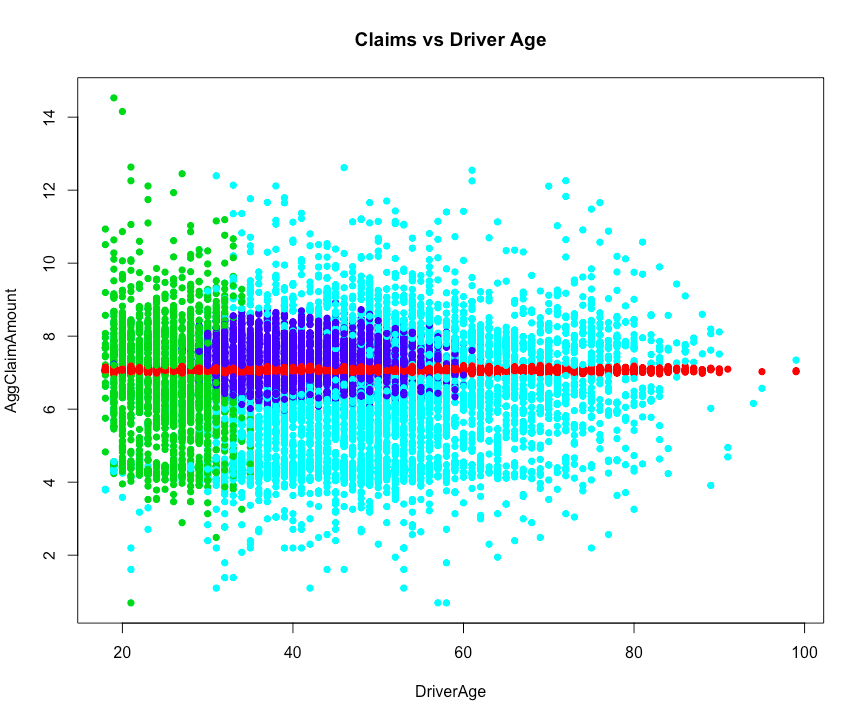
\includegraphics[scale=0.24]{clms.png}
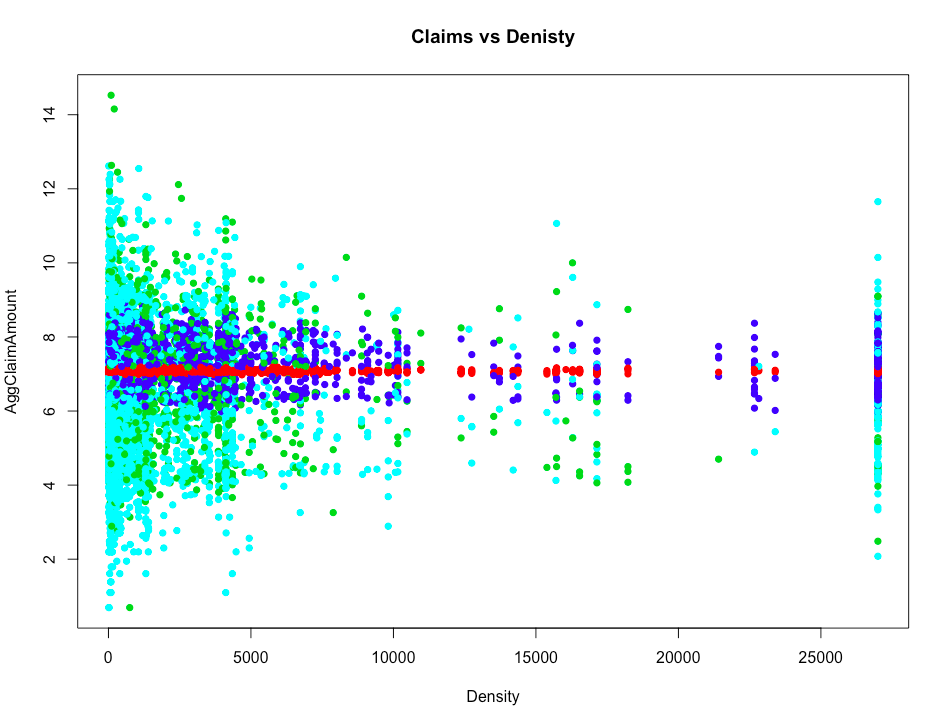
\includegraphics[scale=0.24]{dens.png}
\end{center}
\caption{Claims vs Driver Age: The left figure shows the clusters of claims with respect to driver age as the independent variable . The second figure shows the clusters of claims with respect to Density as the independent variable).}
\label{fig:vet1}
\end{figure}
\begin{table}[!htb]
\centering
\caption{Size of clusters for the GCWM a model.}
\label{table:sizeSev}
\begin{tabular}{cccc}
\hline\hline
1   & 2  &  3   & 4    \\
7119 &1783& 2428& 4060 \\
Red & Green & Teal & Blue \\
\hline\hline
\end{tabular}
\end{table}

After fitting the model, we then take a look at the size of each cluster. The GCWM a function has chosen four components as the best model to represent the data. The size of each cluster is displayed in Table \ref{table:sizeSev}. Attention is brought to largest quantity  of drivers that are grouped into cluster 1. This accounts for $ 46 \% $ of all drivers and is fairly concentrated in both plots in Figure 3.3.
From these results we can create an insurance model with the following characteristics. Cluster 1 drivers have low variability in claims, thus can be insured with a lower upper limit than the other drivers. From a risk management perspective this is the most ideal case as these drivers will claims with very  low variance. Cluster 2 drivers have the second lowest variability, thus we would increase the upper limit. The same can be done for the final two Clusters while adjusting  the limits accordingly.
\begin{table}[!htb]
\centering
\caption{Summarized volatility information of each cluster.}
\label{table:volSev}
\scalebox{0.90}{
\begin{tabular}{llllll}
\hline\hline
Volatility Level - (Cluster)  $\quad$	&		Characteristic     & Minimum & Mean  & Maximum & $\sigma (0.05) $    \\
\hline
	V1 - (1)$\quad\quad\quad$ 	&	Aggregate Claims & 1035    & 1172  & 1340    & \textbf{52.64 }   \\
		&	Driver Age       & 18      & 46.21 & 99      & 15.3     \\
		&	Density          & 3       & 1839  & 27000   & 4546.906 \\
		\hline
	V2 - (4)$\quad\quad\quad$	&Aggregate Claims & 21 & 1823  & 7511  &\textbf{ 1047.06}  \\
	& Driver Age       & 19 & 42.06 & 62    & 7.2      \\
	&  Density          & 3  & 3407  & 27000 & 6618.938 \\
	\hline
V3 - (3)$\quad\quad\quad$	& Aggregate Claims & 2  & 3109  & 301300 & \textbf{ 13468.54} \\
 &Driver Age       & 18 & 52.72 & 99     & 12.6     \\
 & Density          & 2  & 1593  & 27000  & 4310.153\\
\hline
V4 - (2)$\quad\quad\quad$ &Aggregate Claims & 2  & 5043  & 2037000 & \textbf{59750.99} \\
& Driver Age       & 18 & 25.79 & 35      & 4        \\
& Density          & 6  & 2219  & 27000   & 4590.053\\
\hline\hline
\end{tabular}
}
\end{table}
%Volitlity Level 1

%  Aggregate Claims min 1035, mean, 1172 , max  1340 sd \$ 53 %
%  Driver Age min 18  mean 46  max   99.00 , sd 15 years %
% Density   min 3  mean 1839  max 27000  sd 4546.     %


% Voltility Level  2
% Aggregate Claims min 21  mean   1823   max  7511    sd 1047.055
%  Driver Age 18.00   52.72     99.00  sd 12.58355
%  Density 3      221    1593     27000 sd 6618.938



%Volitlity Level 3
%  Aggregate Claims min 2.0 mean  3109.0 max  301300.0 sd 13468
% Driver Age  min 18.00  mean 52.72  max 99.00  sd 12
% Density  min 2    mean 1593   max  27000  sd 4310

% Volitlity Level 4
% Aggregate Claims  min   2 mean  5043  max 2037000 sd  59750.99
% Driver Age 18.00  mean 26   max 35.00  sd 3.95881
% Density min  6   mean  2219  max 27000  sd 4590

\begin{table}[!htb]%Nik: make this a sidewaystable and put it in an appendix	
\begin{adjustwidth}{-2.5cm}{}
\caption{The coefficients and significance  of each cluster.}
\label{table:sevCoef}
\scalebox{0.925}{
\begin{tabular}{|l|rrr|rrr|rrr|rrr|}
\hline\hline
   &  V1           &  (Red)          &              & V2 &  (Blue)          &              & V3 &   (Teal)          &              & V4 & (Green)           &              \\
Coef     & Estimate & Error & P & Estimate    &  Error &P & Estimate   & Error &P  & Estimate    & Error & P \\
\hline
(Intercept)       & $ 7.07 \cdot 10^{0} $ & 1.00       & ***          &  $6.96 \cdot 10^{0} $   & 1.05       & ***          &  $5.92 \cdot 10^{0} $     & 1.12 & ***          & $8.91 \cdot 10^{0}$      & 1.13       & ***          \\
Density           & $1.14 \cdot 10^{-4} $       & 1.00       &              & $ -7.03 \cdot 10^{-3} $     & 1.00       & *            & $-3.47 \cdot 10^{-2} $       & 1.01       & ***          & $3.03 \cdot 10^{-2} $          & 1.01       & ***          \\
DriverAge         & $1.03 \cdot 10^{-4} $   & 1.00       & ***          & $ 9.89 \cdot 10^{-4} $      & 1.00       & .            & $1.88 \cdot 10^{-2} $         & 1.00       & ***          & $-6.39 \cdot 10^{-2} $             & 1.00       & ***          \\
R23 & $4.94 \cdot 10^{-3} $   & 1.00       &              & $-1.39 \cdot 10^{-1} $       & 1.04       & ***          & $1.47 \cdot 10^{-1} $      & 1.12       &              &$-1.91 \cdot 10^{-1} $      & 1.11       & .            \\
R24 & $-1.43 \cdot 10^{-2}$    & 1.00       & ***          & $ 6.58 \cdot 10^{-2} $   & 1.02       & ***          & $-3.61 \cdot 10^{-1} $       & 1.05       & ***          & $-1.71 \cdot 10^{-2} $     & 1.04       &              \\
R25 & $-1.43 \cdot 10^{-2}$  & 1.00       & ***          & $ -1.78 \cdot 10^{-1} $      & 1.04       & ***          & $-1.05 \cdot 10^{-1} $       & 1.09       &              & $1.59 \cdot 10^{-1} $      & 1.09       & .            \\
R31 & $-2.32 \cdot 10^{-3}$   & 1.00       &              & $ 2.43 \cdot 10^{-3} $     & 1.03       &              & $1.98 \cdot 10^{-1} $         & 1.07       & **           & $-8.98 \cdot 10^{-2} $      & 1.06       & .            \\
R52 & $-1.52 \cdot 10^{-2}$      & 1.00       & ***          & $ 2.23 \cdot 10^{-1} $   & 1.02       &              & $-3.89 \cdot 10^{-1} $        & 1.06       & ***          & $1.36 \cdot 10^{-1} $      & 1.06       & *            \\
R53 &  $-1.38 \cdot 10^{-2}$     & 1.00       & ***          & $ 2.22 \cdot 10^{-1} $   & 1.02       & ***          & $-1.78 \cdot 10^{-1} $        & 1.06       & **           & $8.09 \cdot 10^{-2} $      & 1.06       &              \\
R54 &  $-1.47 \cdot 10^{-2}$  & 1.00       & ***          & $ 8.69 \cdot 10^{-4} $   & 1.03       & ***      &    $-4.04 \cdot 10^{-1} $         & 1.08       & ***          & $1.85 \cdot 10^{-1} $        & 1.07       & **           \\
R72 &  $-5.98 \cdot 10^{-3}$   & 1.00       & ***          & $ 1.44 \cdot 10^{-1} $   & 1.03       & ***          & $-6.77 \cdot 10^{-2} $      & 1.07       &              & $2.37 \cdot 10^{-2} $       & 1.06       &              \\
R74 &  $-1.82 \cdot 10^{-2}$      & 1.00       & ***          & $ 1.44 \cdot 10^{-1} $   & 1.06       &              & $-1.05 \cdot 10^{-1} $         & 1.14       &              & $-3.32 \cdot 10^{-1} $    & 1.14       & *            \\
PE    & $-1.21 \cdot 10^{-3}$     & 1.00       &              & $ 3.31 \cdot 10^{-2} $         & 1.02       & ***          & $6.47 \cdot 10^{-2} $       & 1.05       &              & $-1.83 \cdot 10^{-1} $       & 1.04       & ***          \\
PF    & $-2.56 \cdot 10^{-3}$    & 1.00       & *            & $ 7.85 \cdot 10^{-2} $   & 1.02       & .            & $1.43 \cdot 10^{-1} $       & 1.04       & **           & $-3.93 \cdot 10^{-2} $      & 1.04       &              \\
PG    & $-5.31 \cdot 10^{-4}$      & 1.00       &              & $ 1.83 \cdot 10^{-1} $   & 1.02       & ***          & $1.35 \cdot 10^{-1} $        & 1.05       & **           & $-7.17 \cdot 10^{-2} $        & 1.04       & .            \\
PH    & $3.89 \cdot 10^{-3}$     & 1.00       & *            & $ 9.02 \cdot 10^{-2} $   & 1.03       & ***          & $1.15 \cdot 10^{-1} $          & 1.07       & .            & $-1.83 \cdot 10^{-1} $     & 1.07       & **           \\
PI    & $-2.00 \cdot 10^{-3}$      & 1.00       &              & $ 1.20 \cdot 10^{-1} $   & 1.03       & **           & $2.04 \cdot 10^{-1} $        & 1.08       & **           & $-8.05 \cdot 10^{-2} $       & 1.07       &              \\
PJ    & $8.36 \cdot 10^{-3}$       & 1.00       & ***          & $ -5.91 \cdot 10^{-2} $   & 1.03       & ***          & $2.54 \cdot 10^{-1} $        & 1.08       & ***          & $-1.61 \cdot 10^{-1} $          & 1.08       & *            \\
PK    & $5.63 \cdot 10^{-3}$       & 1.00       & *            & $ 6.86 \cdot 10^{-2} $   & 1.04       &              & $1.47 \cdot 10^{-1} $       & 1.09       & .            & $-1.80 \cdot 10^{-1} $      & 1.12       &              \\
PL    & $9.04 \cdot 10^{-3}$     & 1.00       & **           & $ 4.18 \cdot 10^{-1} $   & 1.06       &              & $2.31 \cdot 10^{-1} $          & 1.14       & .            & $3.09 \cdot 10^{-1} $          & 1.18       & .            \\
PM    & $-7.52 \cdot 10^{-3} $  & 1.01       &              & $ 1.14 \cdot 10^{-1} $        & 1.08       & ***          & $-7.67 \cdot 10^{-2} $        & 1.20       &              & $1.68 \cdot 10^{-1} $       & 1.28       &              \\
PN    & $-3.92 \cdot 10^{-3} $    & 1.01       &              &  $ -5.77 \cdot 10^{-1} $   & 1.09       &              & $-4.75 \cdot 10^{-1} $       & 1.24       & *            & $-1.58 \cdot 10^{-1} $      & 1.21       &              \\
PO   & $3.48 \cdot 10^{-3} $    & 1.01       &              & $ 3.57 \cdot 10^{-2} $        & 1.09       & ***          & $1.01 \cdot 10^{-1} $    & 1.23       &              & $-6.48 \cdot 10^{0} $     & 1.63       & ***          \\
C1   & $5.67 \cdot 10^{-3} $  & 1.00       & *            & $ 1.83 \cdot 10^{-1} $        & 1.03       &              & $3.74 \cdot 10^{-2} $         & 1.08       &              & $-2.34 \cdot 10^{-1} $       & 1.08       & **           \\
C2   & $4.58 \cdot 10^{-3} $    & 1.00       & *            &$ 9.89 \cdot 10^{-4} $   & 1.03       & ***          & $-1.02 \cdot 10^{-1} $      & 1.07       &              &  $-5.90 \cdot 10^{-1} $      & 1.07       & ***          \\
C3  & $8.08 \cdot 10^{-3} $   & 1.00       & ***          & $ 1.44 \cdot 10^{-1} $        & 1.03       & ***          & $-1.98 \cdot 10^{-1} $    & 1.07       & **           &  $-5.99 \cdot 10^{-1} $       & 1.07       & ***          \\
C4  & $8.25 \cdot 10^{-3} $  & 1.00       & ***          &$ 2.76 \cdot 10^{-1} $      & 1.03       & ***          &  $-2.21 \cdot 10^{-1} $       & 1.08       & **           & $-3.87 \cdot 10^{-1} $      & 1.09       & ***          \\
C5 & $4.09 \cdot 10^{-3} $& 1.00       & .            & $ 2.09 \cdot 10^{-1} $          & 1.03       & ***          & $-2.13 \cdot 10^{-1} $    & 1.09       & **           & $-9.27 \cdot 10^{-1} $       & 1.09       & ***         \\
\hline\hline
\end{tabular}
}
 \end{adjustwidth}
\end{table}





Table \ref{table:volSev} shows a breakdown of the types of drivers, ordered by volatility in descending order. Beginning with cluster 1, drivers have a mean age of 46 years. The age of these drivers are fairly spread with a standard deviation of 15 years. However, the one noticeable difference is that these drivers tend to have claims between 1035 to 1340, with a standard deviation of 52.64, and a mean of 1172. That means that these drivers rarely exceed costs and tend to have very low volatility. Which implies that claims tend to be the same across all ages. Moving onto to cluster 2, these drivers have the second level of volatility. Drivers in this range tend to have claims anywhere between 21 to 7511,%Nik: 21 and 7511 what? Units should be given, e.g., $, km, etc. 
with standard deviation of 1047, and a mean of 1823. The ages of these drivers are between 19 to 62 with a mean age of 42. One can interpret this cluster as middle aged drivers. The claims of these drivers have higher volatility than the previous cluster, in this case age is very concentrated together with only a standard deviation of just 7 years, in contrast to the previous cluster's standard deviation of 15. Proceeding to the third cluster, its volatility in claims is greater. Drivers in this cluster have claims anywhere between 2 to 301300, with a mean of 3109, and a standard deviation of 13468. The drivers in this cluster are much older than the previous one with a mean age of 52 years and a standard deviation of 12.6. Finally cluster 4 denotes the level of highest volatility. Claims in this cluster of drivers reach the highest cost of 2037000, a mean of 5043, and a standard deviation of 59750.99. Their ages tend to be much younger, with a mean age of 26, and a standard deviation of just 4. This is fairly standard  for car insurance since younger drivers tend to take more risks.

Coefficients of clustered results are used to calculate premiums in car insurance. Table  \ref{table:sevCoef} shows the coefficients of the fitted model. The significance codes are defined as $\approx 0$  (***), 0.001 (**), 0.01 (*), 0.05 (.) %Nik: something wrong here; all of these could be considered $\approx 0$... use < some value.
pertaining to the $p$ value of the specific coefficient. In each cluster significance varies but overall the majority of coefficients are significant. An interpretation of the results is as follows. The first cluster (V1) has significant coefficients of Region (R\#),  Power (P\#), Car age (C\#), and Driver age. We see that the sign of coefficients change depending on the relative center of each cluster. The comparison between driver age in V1 and V4 is a perfect example. The coefficient of driver age is positive in V1 which shows that with larger age, claims tend to go up. Comparing that with last cluster, (V4). The driver age coefficient is negative. This is due to the fact that ages in V4 are very young (mean age of 25). Thus as age increases drivers tend to take less risks and become more responsible, which would decrease cost of claims. We see the same interpretation with Density. Clusters V2, V3, and V4  have density as a significant coefficient. However, the sign of the coefficient changes to negative in V4, while V2 and V3 have positive coefficients. Again this due to the relative centres of the cluster indicate both the magnitude and sign of the coefficient.%Nik: not sure what this means.

To summarize, the drivers have been clustered into four categories with distinct characteristics outlined in Table~\ref{table:volSev}. We have seen how using the results from GCWM a, one can create an insurance model based on clustering algorithms with various levels of risk represented in each cluster. An interesting result was that cluster 1 contradicted the usual understanding that young people take more risks. %Nik: give ref for usual understanding 
The GCWM a method found a group that was the clear majority of drivers, in which the volatility of their claims was extremely low regardless of Driver Age, or Density. This finding shows that GCWM a may potentially find unique models that are otherwise hidden within the data.


 \subsubsection{Modeling Claims Frequency}

In this section, we model frequency of the French motor claims. We consider the covariates log-density, driver age, car age, and a three-class grouping of the power of a car labelled Power F. The choice of covariates stems from the previously modelled single component ZIP \citep{Charpentier:2014}. For the purposes of computational feasibility, only claims from the largest populated insurance region (R24) had been selected. %Nik: is it really infeasible to do more? 
The extension into multiple components is modelled with the linear formula
$$ \text{ Claim Nb $\sim$  Driver Age + Log Density + Car Age + Power F}. $$%Nik: again, I would use a proper equation.

After fitting the model, the size of each cluster is noted. The GCWM a has chosen 3 components as the best model to represent the data. The size of each cluster is displayed in Table~\ref{table:sizeFreq}. %Nik: there is no table with this label...  
Attention is brought %Nik: what does this mean? 
to cluster 2 which holds nearly $67 \%$ of the total population. Cluster 3 holds the fewest amount of drivers with merely $2.4 \% $ of the total population. Table \ref{table:volSev} shows an in-depth analysis of Driver Age and Claim Number as shown in \ref{fig:vet1}.  Cluster 1 has the youngest drivers of the whole population with a mean age of 29.39 and a standard deviation of 4.87. Cluster 2 has a relatively older age group with a mean age of 36.90, and a standard deviation of 1.20. Finally Cluster 3 shows the oldest age group of drivers with a mean age of 54.25 and a standard deviation of 11.66. However when looking at the relative proportion of claims for each cluster as shown in Table \ref{table:claimAn}. One notices that the middle age group has a higher proportion of non-zero claims. Relative to the other clusters, the middle age group has a non-zero claim proportion of 17.25 \%. This is bolded in the Table \ref{table:claimAn} to show the difference of cluster 2 in comparison to 1, and 3.
\begin{figure}[!htb]
\label{figure:3}
\begin{center}
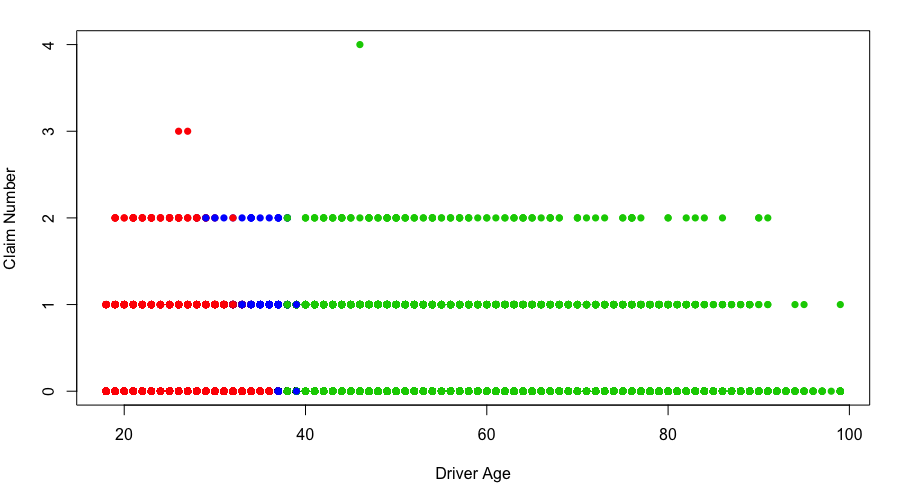
\includegraphics[scale=0.25]{driverVClaimNumber.png}
\end{center}
\caption{Claim number versus driver age, with partitions denoted by colour.}
\end{figure}
\begin{table}[!htb]
\caption{Claim Nb analysis of clusters}
\label{table:claimAn}
\begin{center}
\scalebox{0.90}{
\begin{tabular}{llll}
\hline\hline
Cluster & Claim Nb & Counts & Proportion ($\% $) \\
\hline

1  &    0 & 48172   & 96.98 \%   \\
   &    1 & 1432& 2.90 \%   \\
   &  2 &  64  & 0.12 \%  \\
   &  3 & 2  & $\approx 0 \% $ \\
   \hline
2 &  0 & 3262 & \textbf{82.75 \% } \\
 &   1 & 658 &  \textbf{16.69 \% }\\
 & 2 & 22  & \textbf{0.56 \% } \\
 \hline
3 & 0 & 102905 & 96.18\%   \\
 & 1 & 3963  &  3.71  \% \\
 & 2 & 120 & 0.11 \% \\
 & 4 & 1  & $\approx 0 \% $ \\
 \hline\hline
\end{tabular}
}
\end{center}
\end{table}
\begin{table}[!htb]
\parbox{.45\linewidth}{
\centering
\label{table:2}
\caption{Size of clusters for modelling claims}
\begin{tabular}{ccc}
\hline\hline
1     & 2      & 3    \\
49670 & 106989 & 3942 \\
Red & Green & Blue \\
\hline\hline
\end{tabular}
}
\hfill
\parbox{.45\linewidth}{
\centering
\caption{Driver Age analysis of clusters.}
\label{table:driverFreq}
\begin{tabular}{ccccc}
\hline\hline
Cluster & Minimum & Maximum & Mean & $\sigma$  \\
\hline
 1 &  18 & 38 & 29.39 & 4.87 \\
 2 &  28 & 39 & 36.90 &   1.20 \\
 3 & 38  & 99 & 54.25 & 11.66 \\
 \hline\hline
\end{tabular}
}
\end{table}

The significance of the codes are defined as $\approx 0$  (***), 0.001 (**), 0.01 (*), 0.05 (.) %Nik: same comment as last time
pertaining to the $p$ value of the specific coefficient. For each cluster the significance of the coefficients vary greatly. In cluster 1, the count parameters ($\beta_{xn}$) for the Intercept, Driver Age and Log-Density are highly significant (***). The zero parameters $\beta_{xz}$ are all highly significant with the exception of the power group GH ($\beta_{5z}$). After comparing the zero-inflated model for cluster 2 with a reduced Poisson model, the Vuong statistic had chosen the simpler Poisson model shown in Table~\ref{table:freqCoef}. The Poisson model shows significance for the Intercept, Car Age, and Log-Density. Cluster 3 shows signficance for both zero and count models. The Intercept, Driver Age, and Log Density for both models show high significance.
In summary the drivers have been clustered into three categories outlined in Table~\ref{table:freqCoef}. From the coefficients, one can generate a premium plan tailored to the specific classifications of drivers using GCWM a.
\begin{center}
\begin{flushleft}
\begin{small}
\begin{table}[h!]
\begin{adjustwidth}{-0.5cm}{}
\caption{Table of coefficients for each cluster }%Nik: sidewaystable in appendix
\label{table:freqCoef}
\hspace*{-1cm}\begin{tabular}{|ccccc|cccc|cccc|}
\hline\hline
Par & Est. & Std. Err & Z Val.& P & Est.  & Std. Err & Z Val. & P & Est.  & Std. Err & Z Val. & P \\
\hline
$\beta_{0n}$       & -1.621   & 0.213      & -7.629  & ***   &-3.581	& 0.102	& -35.109	& ***   & 6.973    & 0.923      & 7.553   & ***   \\
$\beta_{1n}$      & -0.075   & 0.006      & -11.631 & ***   & 0.000    & 0.001      & 0.012   &       & -0.220   & 0.028      & -7.773  & ***   \\
$\beta_{2n}$      & -0.006   & 0.005      & -1.181  &       & -0.015	& 0.003	& -5.481 & 	***   & 0.003    & 0.009      & 0.325   &       \\
$\beta_{3n}$       & 0.113    & 0.015      & 7.589   & ***   &0.085 & 	0.010 & 	8.884	& ***  & 0.103    & 0.030      & 3.401   & ***   \\
$\beta_{4n}$   & -0.065   & 0.086      & -0.752  &       & 0.094    & 0.054      & 1.611  &    & -0.087   & 0.153      & -0.570  &       \\
$\beta_{5n}$   & 0.081    & 0.092      & 0.875   &       & 0.074    & 0.058      & 1.287   &       & -0.006   & 0.167      & -0.039  &       \\
$\beta_{0z}$   & -228.080 & 55.429     & -4.115  & ***   & &     &    &      & -106.767 & 6.873      & -15.534 & ***   \\
$\beta_{1z}$  & 7.601    & 1.832      & 4.149   & ***   &  &       & &       &3.059   &  0.194    & 15.782   & ***   \\
$\beta_{2z}$    & -0.313   & 0.128      & -2.447  & *     &   &     &   &  & 0.017    & 0.019      & 0.921   &       \\
$\beta_{3z}$  & -4.309   & 1.002      & -4.303  & ***   &   &     &   &     & -1.133   & 0.087      & -12.967 & ***   \\
$\beta_{4z}$ & 7.891    & 2.105      & 3.750   & ***   &    &      &   &       & -0.094   & 0.313      & -0.301  &       \\
$\beta_{5z}$     & -1.267   & 1.346      & -0.941  &       &    &    &  &       & 0.096    & 0.334      & 0.288   &   \\
\hline\hline
\end{tabular}\hspace*{-1cm}
\end{adjustwidth}
\end{table}
\end{small}
\end{flushleft}
\end{center}

%Nik, a general comment: please be careful with consistency of notation. For instance, p or P for $p$-value?

\section{Simulation Study}

Two simulation studies are conducted to determine the validity of transformation and the effectiveness of the Bernoulli-Poisson partitioning method. The first section outlines the need for transformation in the covariates. The second section shows the classification accuracy and other relevant analysis for the Bernoulli-Poisson method.


\subsection{Simulation Study - Transformation}


In this section, we show how the proposed methodology works for different simulation settings. The simulation study was generated based on the regression coefficients of the \textbf{CASdataset} used in the previous section. The aim of the simulation study was to test the accuracy and ability of both GCWM a and CWM to return estimates of true parameters when one or more of the covariates is lognormal and the other two are Gaussian. This was designed to test both functions in the event when one of the covariates is non-Gaussian. The motivation behind this is fact is that many covariates used in insurance are likely to come from non-Gaussian distribution. Thus this was aimed to test the relevancy of CWM, which treats all covariates as Gaussian.

We define Model 1 as the base line model in which the coefficients were generated for \textbf{CASdataset} and reported in upper portion of Table 2. These coefficients were then rounded and treated as true parameters. A simulation with three GLM mixture components was then generated around these true parameters in which the third covariate $X_3$ was lognormal. Stemming from this, both CWM and  GCWM a were run. The  GCWM a treats $X_3$ as a lognormal covariate which then applies the relevant transformation.

The results for Model 1 were summarized in upper portion of Table 3 based on the performance of the  GCWM a approach. The simulation was run $1000$ times. We reported the percentage of runs for each predictor and the corresponding intercept in each mixture component under the assumption of $5\%$ error. For example, predictor $X_2$ in the component 2 of Model 1 reported $90.10\%$ accuracy. This means that $90.1\%$ of the time the true parameter was estimated within $5\%$ error. In this setting, predictor $X_1$ in the second component was insignificant in the real data set. The purpose of including this parameter in Model 1 was to test the sensitivity of  GCWM a for insignificant predictors. In this case, the result of zero is underlined and it means that it has no influence on the response variable in this simulation.Further, we created Models 2, 3, 4 and 5 by altering the parameters of Model 1 by $+30\%$, $-30\%$, $+50\%$, and $-50\%$ accordingly and keeping the second covariate of the second component as an insignificant predictor form the \textbf{CASdataset} model. This was done to test the accuracy of  GCWM a to the  sensitivity of coefficients. Based on the results in Table 3, we can see that  GCWM a performs well for all simulation settings.




\begin{center}
\begin{table}[!htb]
\label{my-label}
\caption{GCWM a vs CWM Accuracy: Covariate $X_3$ is treated as log-normal, the rest are Gaussian covariates. The transformation of $X_3$ is considered.}
\begin{adjustwidth}{-1cm}{}
\begin{tabular}{|rrrrrr|rrrr|}
\hline\hline
Model & Component & Intercept & $X_1$ &$X_2$ & $X_3$& Intercept & $X_1$ &$X_2$ & $X_3$  \\
\hline
1     & 1         & 93.00\%   & 90.10\%  & 93.00\%  & 93.10\% & 0.00\% & 0.00\% & 0.00\% & 0.00\%   \\
      & 2         & 90.10\%   & \underline{0.00\%}   & 90.10\%  & 90.10\% & 0.00\% & 0.00\% & 0.00\% & 0.00\%  \\
      & 3         & 99.20\%   & 99.10\%  & 99.20\%  & 99.20\% & 0.00\% & 0.00\% & 0.00\% & 0.00\%  \\ 
2     & 1         & 89.80\%   & 89.20\%  & 89.80\%  & 89.80\% & 0.00\% & 0.00\% & 4.60\% & 0.00\%  \\
      & 2         & 89.20\%   &\underline{0.00\%}   & 89.20\%  & 89.20\% & 0.00\% & \underline{0.00\%} & 0.00\% & 0.00\%   \\
      & 3         & 99.20\%   & 99.20\%  & 99.20\%  & 99.20\% & 0.00\% & 0.20\% & 1.70\% & 0.00\%  \\ 
3     & 1         & 100.00\%  & 100.00\% & 100.00\% & 100.00\%  & 0.00\% & 0.00\% & 0.00\% & 0.00\% \\
      & 2         & 100.00\%  & \underline{0.00\%}   & 100.00\% & 100.00\% & 0.00\% & 0.00\% & 0.00\% & 0.00\% \\
      & 3         & 99.20\%   & 99.20\%  & 99.20\%  & 99.20\%  & 0.00\% & 0.00\% & 0.00\% & 0.00\%\\ 
      4 & 1 & 88.60\% & 86.80\% & 88.60\% & 87.00\%  & 0.00\% & 0.00\% & 0.00\%  & 0.00\%  \\
  & 2 & 86.90\% &\underline{ 0.00\%}  & 86.90\% & 86.90\% & 0.00\% & \underline{0.00\%} & 0.00\%  & 0.00\%  \\
  & 3 & 99.20\% & 99.20\% & 99.20\% & 99.20\% & 0.00\% & 0.00\% & 0.00\%  & 0.00\% \\ 
5 & 1 & 85.90\% & 84.90\% & 85.60\% & 85.90\% & 0.00\% & 0.00\% & 0.00\%  & 0.00\% \\
  & 2 & 85.00\% &\underline{ 0.00\%}  & 84.90\% & 84.90\% & 0.00\% & \underline{0.00\%} & 0.00\%  & 0.00\%  \\
  & 3 & 99.20\% & 99.20\% & 99.20\% & 99.20\% & 0.00\% & 0.20\% & 10.90\% & 0.00\% \\
      \hline\hline
\end{tabular}
\end{adjustwidth}
\end{table}
\end{center}


Table 4 provides the summary of the results when CWM was used in the analysis of the same models considered in Table 3. It is not surprising to see that barely any of the simulation runs estimated correctly all parameters as most of the results are zero. This means that the performance of CWM approach is poor in presence of one non-Gaussian covariate which in this case is a log-normal covariate. Similarly to Table 3, Table-4 shows the underlined results pointing to insignificant predictors.

\begin{table}[!htb]
\centering
\caption{ GCWM a results: the summary of MSE for all parameters used in five models. The covariate $X_3$ is treated as log-normal a nd the rest are Gaussian. These results correspond to those in Table 3.}
\label{my-label}
\begin{tabular}{rrrrrrrrrr}
\hline\hline
Model & Component & $\beta_o$ &  MSE($\beta_o$)   &  $\beta_1$ & MSE($\beta_1$)& $\beta_2$ &MSE($\beta_2$)   & $\beta_3$ &  MSE($\beta_3$)  \\
\hline
1     & 1         & 1028& (11.353)   & 0.03& (0.00)  & 3.5& (0.00)    & -380& (0.09)   \\
      & 2         & 1600& (0.000)     & -0.01&(0.00) & 1.5&(0.00)    & -250&(0.00)   \\
      & 3         & 40000&(0.035)    & -6.00&(0.00) & -305&(0.00) & 1100&(0.47)   \\
2     & 1         & 1350&(0.167)     & 0.04&(0.00)  & 4.5&(0.00)    & -500&(0.03)   \\
      & 2         & 2080& (0.001)     & 0.04&(0.00)  & 2.0&(0.00)    & -325&(0.00)   \\
      & 3         & 52000& (0.012)    & -8.00&(0.00) & 450&(0.00)  & 14300&(0.01)  \\
3     & 1         & 720& (0.001)      & 0.02&(0.00)  & 2.5&(0.00)   & -266&(0.00)   \\
      & 2         & 1100& (0.008)     & 0.00&(0.00)  & 1.1&(0.00)    & -17511&(0.00) \\
      & 3         & 28000& (0.002)    & -4.20&(0.00) & 245&(0.00)  & 7700.&(0.00) \\
4     & 1         & 1650&(13.056)   & 0.05&(0.00)  & 5.3&(0.00)    & -570&(0.00)   \\
      & 2         & 2400& (0.000)     & -0.01&(0.00) & 2.3&(0.00)    & -375&(0.00)   \\
      & 3         & 60000& (0.051)    & -9.00&(0.00) & -457&(0.00) & 16500&(0.00)  \\
5     & 1         & 500& (1.115)     & 0.02&(0.00)  & 2.0&(0.00)    & -190&(0.05)   \\
      & 2         & 800& (0.003)      & 0.00&(0.00)  & 0.8&(0.00)    & -120&(0.00)   \\
      & 3         & 20000& (0.000)    & -3.00&(0.00) & -150&(0.00) & 5500&(0.00)  \\
      \hline\hline
\end{tabular}

\end{table}







Table 5 provides the summary of Mean Squared Errors (MSE) of each parameter of the models in Table 3 estimated via 1000 simulation runs. The MSE is computed using the following formula MSE$(\beta_i) = \frac{\sum_i^n (\beta_i - \hat\beta_i ) ^2}{n}$. The MSEs related to the predictor variables for all models and their corresponding components are about zero indicating that  GCWM a approach performs well. This is also a result of having a small size coefficients.


\begin{table}[!htb]
\centering
\caption{CWM results: the summary of MSE for all parameters used in five models. All three covariates are treated as Gaussian. These results correspond to those in Table 4.}
\label{my-label}
\begin{tabular}{rrrrrrrrrrrr}
\hline\hline
Model & Component & $\beta_o$ &  MSE($\beta_o$)   &  $\beta_1$ & MSE($\beta_1$)& $\beta_2$ &MSE($\beta_2$)   & $\beta_3$ &  MSE($\beta_3$)  \\
\hline
1     & 1         & 1028& ($\cdot$)   & 0.03&  ($\cdot$)   & 3.5&  ($\cdot$)    & -380&  ($\cdot$)    \\
      & 2         & 1600&  ($\cdot$)      & -0.01& ($\cdot$)  & 1.5& ($\cdot$)     & -250& ($\cdot$)  \\
      & 3         & 40000& ($\cdot$)     & -6.00& ($\cdot$)  & -305& ($\cdot$)  & 1100& ($\cdot$)    \\
2     & 1         & 1350& ($\cdot$)     & 0.04& ($\cdot$) & 4.5& ($\cdot$)    & -500& ($\cdot$)  \\
      & 2         & 2080&  ($\cdot$)    & 0.04& ($\cdot$)   & 2.0& ($\cdot$)     & -325& ($\cdot$)   \\
      & 3         & 52000&  ($\cdot$)     & -8.00& (0.006)  & 450& (44.1)   & 14300& ($\cdot$)  \\
3     & 1         & 720&  ($\cdot$)     & 0.02& ($\cdot$)   & 2.5& ($\cdot$)    & -266& ($\cdot$)    \\
      & 2         & 1100&  (65.814)     & 0.00& ($\cdot$)   & 1.1& ($\cdot$)     & -17511& ($\cdot$)  \\
      & 3         & 28000& ($\cdot$)   & -4.20& ($\cdot$)  & 245& ($\cdot$)   & 7700.& ($\cdot$)  \\
4     & 1         & 1650& ($\cdot$)    & 0.05& ($\cdot$)  & 5.3& ($\cdot$)    & -570& ($\cdot$)  \\
      & 2         & 2400&  ($\cdot$)     & -0.01& ($\cdot$)  & 2.3& ($\cdot$)    & -375& ($\cdot$)    \\
      & 3         & 60000&  ($\cdot$)     & -9.00& ($\cdot$)  & -457& ($\cdot$)  & 16500& ($\cdot$)   \\
5     & 1         & 500&  ($\cdot$)     & 0.02& ($\cdot$)   & 2.0& ($\cdot$)   & -190& ($\cdot$)  \\
      & 2         & 800&  ($\cdot$)      & 0.00& ($\cdot$)   & 0.8& ($\cdot$)    & -120& ($\cdot$)  \\
      & 3         & 20000&  ($\cdot$)     & -3.00& (0.003)  & -150& (4.7) & 5500& ($\cdot$) \\
      \hline\hline
\end{tabular}
\end{table}








Table 6 provides the summary of Mean Squared Errors (MSE) of each parameter of the models in Table 4 estimated via 1000 simulation runs.
In contrary to the results reported in Table 5, these results in Table 6 are significantly different. We can observe that the MSEs for most of the Models and their corresponding components are not generated at all and as such they are shown as $(\cdot)$. This is not surprising because Table 4 shows the accuracy of CWM is not good when attempting to model non-Gaussian predictors as Gaussian.

In summary, our simulation results showed good performance of  GCWM a approach in modeling non-Gaussian covariates. More specifically, these results show high accuracy when covariates are log-normal. In contrary, CWM fails to estimate parameters accurately when the Gaussian assumption is violated.

\subsection{Simulation Study - Bernoulli-Poisson Partitioning}

In this section we show how the Bernoulli-Poisson partitioning (BP) method  behaves under different conditions. The components were genereated under similar coefficients taken from the \textbf{CASDatasets} package. The coefficients were rounded and treated as true parameters to which data was generated from. The mean and standard deviation of the covariates within each component was also taken into account when generating data. The first simulation examines the performance of the GCWM a model for classification. We generate three components each with sample size $N=1000$ for a total of $3000$ simulated points.
The model generated is similar to the mean and standard deviations of Table \ref{table:driverFreq}. Consider three simulated covariates and the following GLM model
$$ \text{SimClaims} \sim \text{SimDriverAge + SimLogDensity + SimCarAge} . $$
 Here the GCWM a model is fitted to the simulated data and used to classify into three components. The misclassification rate is calculated by the proportion of true labels placed in other components by the GCWM a model.  The results of the simulation is based on the generated dataset are presented in Table \ref{table:driverFreq}. The total misclassification rate  is $1.8 \% $ and the majority of misclassified components are between components two and three.
\begin{table}[!htb]
\begin{center}
\caption{Misclassfication rate and label comparison of generated data.}
\begin{tabular}{c c c c c c}
\hline\hline 
    True Labels       &  \multicolumn{3}{c}{ Classified }   & Misclassification Rate (\%) &  \\ \cmidrule{2-4}
   & 1                              & 2   & 3   &                            &  \\ \hline
1              & 992                            & 3   & 5   & 0.80                      &  \\
2              & 0                              & 990 & 10  & 1.00                       &  \\
3              & 15                             & 20  & 965 & 3.50                      &  \\  \hline 
                \multicolumn{4}{l}{Overall Misclassification Rate}        & 1.80 \%                     & \\
        		\multicolumn{4}{l}{Average Purity} & 98.23 \%  \\
                \multicolumn{4}{l}{Adjusted Rand Index} & 0.9479 &  \\
    \hline\hline  
\end{tabular}
\end{center}
\begin{align*}
n_{ij} &= \text{ across diagonal }, \quad\quad  a_i = \text{ row sums }, \quad\quad b_j = \text { column sums } \\
 ARI &= \frac{ \sum_{ij} \binom{n_{ij}}{2} - [\sum_i \binom{a_i}{2} \sum_j \binom{b_j}{2}] / \binom{n}{2} }{ \frac{1}{2} [\sum_i \binom{a_i}{2} + \sum_j \binom{b_j}{2}] - [\sum_i \binom{a_i}{2} \sum_j \binom{b_j}{2}] / \binom{n}{2} } \quad\quad AP = \frac{1}{N} \sum_i  n_{ij}  
\end{align*}
\end{table}

The experiment is expanded further to show how Bernoulli-Poisson partitioning behaves over 1000 runs and under two different conditions. The first condition is defined as follows. The mean and standard deviations are taken as given by the estimated  ZIP components from the \textbf{CASDataset}. The second condition involves adjusting the means of two of the covariates so they are closer to each other. The goal is to show that the BP-method holds its use even when means among covariates are close.  Conditions are divided into two categories. N is considered normal, where the covariate means are taken directly from the sample data. C is considered to be ``close", where the covariate means are manipulated so that they are closer to each other within some degree. This is a common problem in classification where if the means among two different components are close, then misclassification rate increases [\cite{LimHwa}]. Experiment 2 defines the use of 3 different partitioning methods to initialize a zero-inflated model. Poisson method assumes that the presence of non-zeros will provide a better partitioning of the data-set. Bernoulli assumes that the presence of excess zeros will determine the best partitioning of the data-set . Finally the BP-Method assumes that both methods are weighed equally and therefore both must be taken into account when partitioning the dataset. The mean and standard deviation of each measurement is provided in Table \ref{table:exper2}.

\begin{table}[!htb]
\begin{center}
\caption{Experiment 2: mean and standard deviations for each statistic comparing each method.}
\label{table:exper2}
\begin{tabular}{lllll}
\hline\hline
Type   & Condition & Poisson  ($\sigma $) & Bernoulli  ($ \sigma $) & BP-Method ($ \sigma $) \\
\hline
Misclassification Rate& N         & 1.70\%  (6.00)       & 1.60\% (6.00)         & 1.10\% (0.02)         \\
       & C         & 5.00\%  (7.00)       & 6.00\% (2.00)         & 7.00\% (4.00)         \\
Average Purity & N         & 98.87\% (2.00)    & 98.91\% (2.25)      & 99.18\% (0.81)     \\
       & C         & 95.38\% (4.00)    & 94.55\% (1.00)      & 96.95\% (0.48)      \\
Adjusted Rand Index  & N         & 0.9662 (0.07)    & 0.9677  ( 0.07)     & 0.9729 (0.0217)      \\
       & C         & 0.8706 (0.08)    & 0.8366 (0.04)      & 0.8538 ( 0.0453) \\
       \hline\hline
\end{tabular}
\end{center}
\end{table}
Several findings are concluded from Table \ref{table:exper2}. Under condition N, the BP method shows better performance in error and is found to be less sensitive than other methods with an error rate of $ 1.10 \% $ and a standard deviation of $ 0.02 \% $.  Further findings show that when condition C is imposed then Bernoulli has better performance in terms of findings. The ARI shows good measurements overall however the BP-Method under condition N has a very good ARI with a small standard deviation. The Average Purity of the BP-Method is the best out of all other methods, which is relevant to estimating coefficients accurately for the ZIP optimization.

\section{Conclusion}

In this paper, we extend the class of generalized linear mixture CWM models by accomplishing two main goals. First, we propose the methodology that allows for continuous covariates to follow a non-Gaussian distribution. Imposing Gaussian distribution on a skewed data may result in an suboptimal model fit. Second, we propose a new Poisson CWM methodology that uses Bernoulli-Poisson partitioning and allows for implementation of zero-inflated Poisson CWM model. We call our proposed model class GCWM a which reflects two extensions made to the existing CWM class of models.

The GCWM a models allows for great applications in predictive modeling of insurance claims by overcoming a few limitations of the current CWM models. Zero-inflated GCWM a allows for finding clusters within claims frequency which is an important information in risk classification and modeling of claims frequency. Further, some insurance rating variables used in the predictive modeling of severity claims may not strictly follow Gaussian assumptions, e.g. driver's age or car age (treated as continuous covariates). An adequate transformation can be considered on the continues covariates to relax current assumptions and improve the model fit. We demonstrated that if there is a need for transformation, a Lognormal transformation can be considered easily to improve the model fit. 

The results of our extensive simulation study showed the excellent performance of the proposed model in case of modeling non-Gaussian covariates. We found  that current CWM model fails to estimate the parameters accurately when the Gaussian assumption is violated. The GCWM a shows significant improvement in the model fit over the CWM model based on AIC and BIC criteria. We also tested Bernoulli-Poisson partitioning of zero-inflated GCWM a under different conditions and found that our proposed partitioning method has a very low misclassification rate, high average purity, and high average rand index.

Our approach is relevant to the actuarial pricing and risk management when current practices are based on implementation of various GLM models. Further extension of this work may incorporate Bayesian setting by exploring different assumption on informative and noninformative priors (see \cite{Ibrahim+Laud:1991}). By utilizing these techniques actuaries will be able to make inferences from posterior distributions of model parameters and from predictive distributions in order to improve pricing and risk management of the insured portfolio. 
\newpage
\section{Appendix}

\subsection{Derivation of the Log-normal Distribution }
Consider a random variable $U$ which has univariate Log-normal distribution, with $u \in \mathbb{R}^+$, and which has parameters $\mu \in \mathbb{R}, \sigma \in \mathbb{R}^+ $. The density of random variable $U$ is then defined  as
$$\mathcal{LN}(u; \mu, \sigma)dx = \frac{1}{u\sigma\sqrt{2\pi}}\exp\left[-\frac{(\ln u - \mu)^2}{2\sigma^2}	\right].$$ 
For full definition of lognormal distribution see for example pg. 14 of \cite{johnson1995continuous}. If random variable $X$ is normally distributed ie. $ X \sim \mathcal{N}(x; \mu, \sigma) $, then $U = \exp{(X)}\sim \mathcal{LN}(u; \mu, \sigma) $. 
\begin{proof}
Let $p_U(u)$, and $ p_X(x) $ be the probability density function of $U$ and $X$ respectively. By the change of variables theorem (\cite{murphy2012machine} section 2.6.2.1) the density $p_U(u)$ is derived to be
$$p_U(u) = p_X(\ln u )\frac{\partial}{\partial u} \ln u  =  p_X(\ln u ) \frac{1}{u} =  \frac{1}{u\sigma\sqrt{2\pi}}\exp\left[-\frac{(\ln u - \mu)^2}{2\sigma^2}	\right].$$
\end{proof}
We can extend to a Log-normal multivariate case where the random variable $\bm{U} $, $\bm{u} \in \mathbb{R^{+}}^p $, parameterized by $ \bm{\mu} \in \mathbb{R}^p, \bm{\Sigma} \in  \mathbb{R^{+}}^p \label{changeVarUni} $, $p \in \mathbb{N}$ denoting the p-dimensional space, and the density as
$$ f^U(\bm{u}; \bm{\mu } , \bm{\Sigma} )= \frac{1}{(\prod_{i=1}^{N}u_{i})| \bm{\Sigma} |(2 \pi)^{\frac{p}{2}}}   \exp\left[-\frac{1}{2}(\ln \bm{u} -\bm{\mu})^{'}  \bm{\Sigma^{-1}}(\ln \bm{u} -\bm{\mu})\right].  $$

Similarly to above we let the random variable $\bm{X} \sim \mathcal{MVN}(\bm{x}, \bm{\mu},\bm{\Sigma}) $ (distributed multivariate normal) , then $\bm{U} = \exp(\bm{X} ) \sim  f^U(\bm{u}; \bm{\mu } , \bm{\Sigma} )$.  

\begin{proof}
Let $f^U(\bm{u}; \bm{\mu},\bm{\Sigma})$ and $f^X(\bm{x}; \bm{\mu},\bm{\Sigma})$ be the probability density functions of $\bm{U}$ and $\bm{X}$ respectively. By the multivariate change of variables theorem (\cite{murphy2012machine} section 2.6.2.1), we derive the lognormal distribution, where $ | \det J_{\ln} (u) | $ is the absolute value of the determinant for the Jacobian of the multivariate transformation $\ln(\bm{U}) = \bm{X} $. 
\begin{align*}
 | \det J_{\ln} (\bm{u}) | & = \prod_{i=1}^n u_i^{-1}, \\
 f^U(\bm{u}; \bm{\mu},\bm{\Sigma})  & =  f^X(\ln \bm{u}; \bm{\mu},\bm{\Sigma})  | \det J_{\ln} (u) | \\
  & = f^X(\ln \bm{u}; \bm{\mu},\bm{\Sigma})\prod_{i=1}^n u_i^{-1} \\
  & =  \frac{1}{(\prod_{i=1}^{N}u_{i})| \bm{\Sigma} |(2 \pi)^{\frac{p}{2}}}   \exp\left[-\frac{1}{2}(\ln \bm{u} -\bm{\mu})^{'}  \bm{\Sigma^{-1}}(\ln \bm{u} -\bm{\mu})\right].  
  \end{align*}
\end{proof}

\bibliographystyle{elsart-harv}
\bibliography{GLM_Mixtures_2018}

\end{document}


